\uuid{AdEa}
\exo7id{7156}
\titre{exo7 7156}
\auteur{megy}
\organisation{exo7}
\datecreate{2017-05-13}
\isIndication{true}
\isCorrection{true}
\chapitre{Géométrie affine euclidienne}
\sousChapitre{Géométrie affine euclidienne du plan}
\module{Géométrie}
\niveau{L2}
\difficulte{}

\contenu{
\texte{
% concours général 88, cocyclicité, angle d'une similitude directe
Soient $M$, $M_1$, $M_2$, $M_3$ et $M_4$ cinq points distincts sur un cercle $\mathcal C$. Montrer que le produit des distances de $M$ aux droites $(M_1M_2)$ et $(M_3M_4)$ est égal au produit des distances de $M$ aux droites $(M_1M_3)$ et $(M_2M_4)$.
\begin{center}
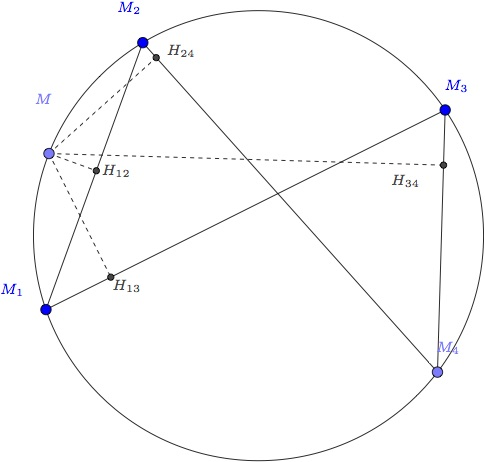
\includegraphics{../images/AdEa-1}
\end{center}
}
\indication{Reformuler une égalité de produits en une égalité de quotients.

Utiliser des similitudes de centre $M$.}
\reponse{
Soient $H_{12}$, $H_{34}$, $H_{13}$ et $H_{24}$ les projetés orthogonaux de $M$ sur les droites $(M_1M_2)$, $(M_3M_4)$, $(M_1M_3)$ et $(M_2M_4)$. Soit $s$ la similitude directe de centre $M$ qui envoie $M_2$ sur $M_3$. L'image par $s$ de la droite $(M_1M_2)$ est une droite $\mathcal D$ passant par $M_3$ et telle que 
\[ (M_1M_2,\mathcal D)=(MM_2,MM_3).\]
Or, on a $(MM_2,MM_3)=(M_1M_2,M_1M_3)$ car les quatre points sont cocycliques. On en déduit que $\mathcal D = (M_1M_3)$, et donc que $s$ envoie la droite $(M_1M_2)$ sur la droite $(M_1M_3)$.

On prouve de la même manière que $s$ envoie la droite $(M_2M_4)$ sur la droite $(M_3M_4)$.

Comme $s(M)=M$ et que les similitudes conservent les angles orientés et en particulier l'orthogonalité, on en déduit que $s(H_{12})=H_{13}$ et que $s(H_{24})=H_{34}$.

Comme une similitude conserve les rapports de longueurs, on a finalement
$\frac{MH_{13}}{MH_{34}} = \frac{MH_{12}}{MH_{24}}$ c'est-à-dire  :
\[
MH_{12} \cdot MH_{34} = MH_{13}\cdot MH_{24}.
\]
}
}
